\documentclass[14pt]{extarticle}
\usepackage{graphicx}
\usepackage{hyperref} 
\usepackage{enumitem}
\usepackage{makecell}
\usepackage{amsmath}
\usepackage{amssymb}
\usepackage{gensymb}
\usepackage[T1]{fontenc}
\usepackage{fancyhdr}
%\usepackage[shortlabels]{enumerate}

\graphicspath{ {/home/nareshguru77/Documents/learning_materials/Semester_2/RandD/Semantic_Segmentation/first_report} }

\usepackage[letterpaper, portrait, margin=0.8in]{geometry}

\pagestyle{fancy}
\fancyhf{}
%\rhead{Share\LaTeX}
\lhead{Semantic Segmentation}
\rfoot{Page \thepage}
\lfoot{ HBRS [MAS WS17-18]}


\begin{document}

\begin{center}
\begin{Large}

\underline{\textbf{R\&D meeting}}\\
\vspace{3mm}
\today
\vspace{3mm}

\textbf{Semantic Segmentation using Resource Efficient Deep Learning}

\end{Large}
\end{center}

\section{Approach selection:}
\subsection{Semantic segmentation models:}

\begin{figure}[!htb]
	\centering
	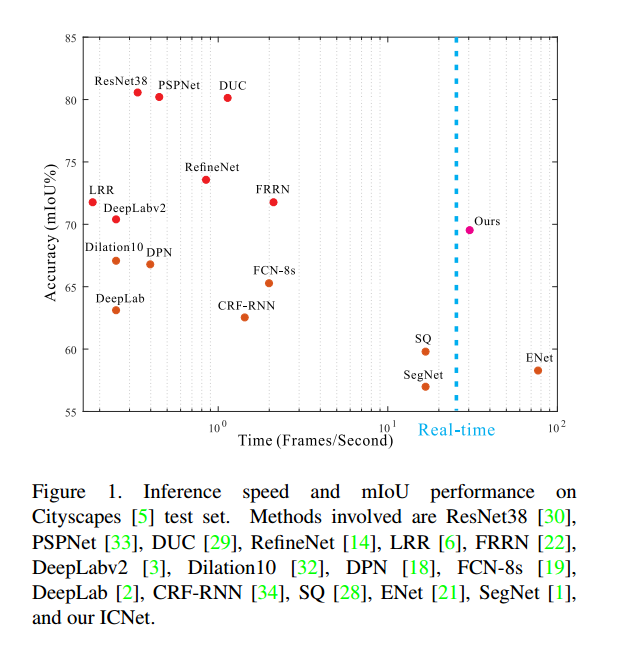
\includegraphics[scale=0.6]{from_icnet}
\end{figure}

Leaderboard changes in Cityscapes testset. (DeepLabv3)

\subsection{Resource efficiency:}
\begin{itemize}
	\item Pruning.
	\item Depthwise separable convolutions like in MobileNet.
	\item Hashing trick.
	\item Rank regularization.
\end{itemize}

\section{Annotation tools:}
\begin{itemize}
	\item LabelMe: web based tool is public and data would also be public.
	\item LabelMe Matlab toolbox: yet to try..
	\item University bonn annotation tool:
	\item Pixel annotation tool (using watershed algorithm): works in windows. Seems to be useful.
	\item Ratsnake: tool dint seem to be useful although the website had options like superpixel suggestions.
	\item LabelImg: Can be used but time consuming.
	\item Figi: used in medical image segmentation. Has many options. Still exploring.
\end{itemize}

\section{Dataset:}
\begin{itemize}
	\item 
	\item 
	\item Are the images expected to be common for the deep learning R\&D (same dataset images but different annotations specific to be R\&D)..?
\end{itemize}

\section{Paper collection:}
\begin{itemize}
	\item Many relavant papers.. All of them need to be read?
\end{itemize}


%\begin{thebibliography}{9}

%\bibitem{1}

%\end{thebibliography}

\end{document}